% Felipe Bandeira da Silva

%\documentclass[a4paper, 10pt]{article}
\documentclass[paper=a4, fontsize=11pt]{article}

\usepackage[brazil]{babel}
\usepackage[utf8]{inputenc}
\usepackage{listings}
\usepackage{color}
\usepackage{amsthm}
\usepackage{graphicx}

%\usepackage{schemabloc}
%\usetikzlibrary{circuits}

\setlength{\parindent}{0pt}
\setlength{\parskip}{18pt}

\renewcommand{\labelitemi}{$-$}

\begin{document}


Como já é de conhecimento de todos, os testes feitos no ''formigueiro'' apresentam
resultados estranhos e totalmente incoerentes. Ensaios estes que 
são realizados utilizando os seguintes equipamentos(todos conectados na mesma fonte, 220V):
\begin{itemize}
    \item Fonte Geradora de Alta Tensão(desenvolvida por: LCE, LAMOTRIZ)
\item Sistema de aquisição(Agilent U2535, Sensor de corrente(Hall) e Tensão, Netbook)
\item Osciloscópio(ponteira de alta tensão e ponteira de corrente, usado apenas 
para comparação com o software Labview.
\end{itemize}

Lembrando, os ensaios realizados na Hidráulica e no estacionamento do DEE 
apresentam resultados coerente. O sinal é considerado coerente quando a forma de onda
medida pelos instrumentos, pode ser representada pela equação 1. Equação esta que 
não leva em consideração os efeitos indutivos e capacitivos. 

\begin{equation}
v(t) = V_p e^{-t/\tau}
\end{equation}

Onde $V_p$ representa a tensão de pico da fonte, em torno de $810 V$. A constante
$\tau$ é dependente da resistência de Thevenin vista pela fonte, pontos A e B, mostrados
na figura 1. Para uma resistência de 100 $\Omega$ entre os pontos A e B, considerando
uma capacitância de 1.1 $\mu F$
o circuito  deve responder de tal forma, que é necessário 550 $\mu s$ para o 
descarregamento de  99 $\%$ do capacitor. A figura 2 representa graficamente a situação.

\begin{figure}[!ht]
    \centering
    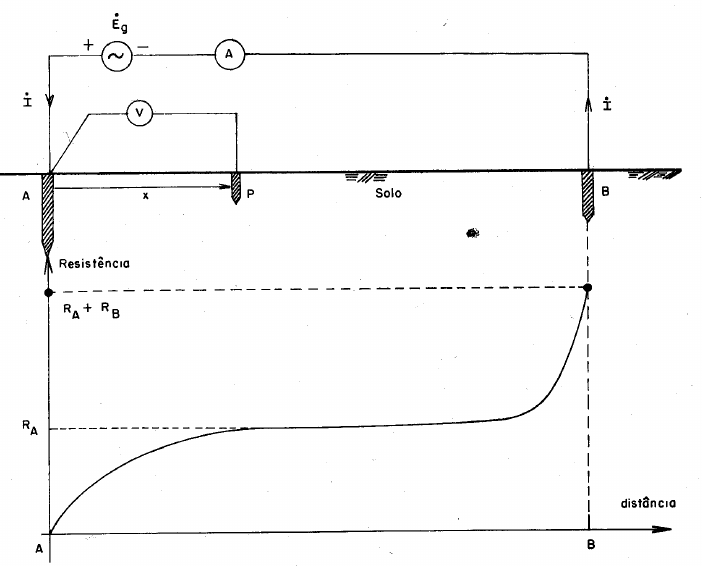
\includegraphics[scale=.6]{medicao.png}
    \caption{Curva de Resistência de Terra x Distância, Fonte: Kinderman}
\end{figure}

\begin{figure}[!ht]
    \centering
    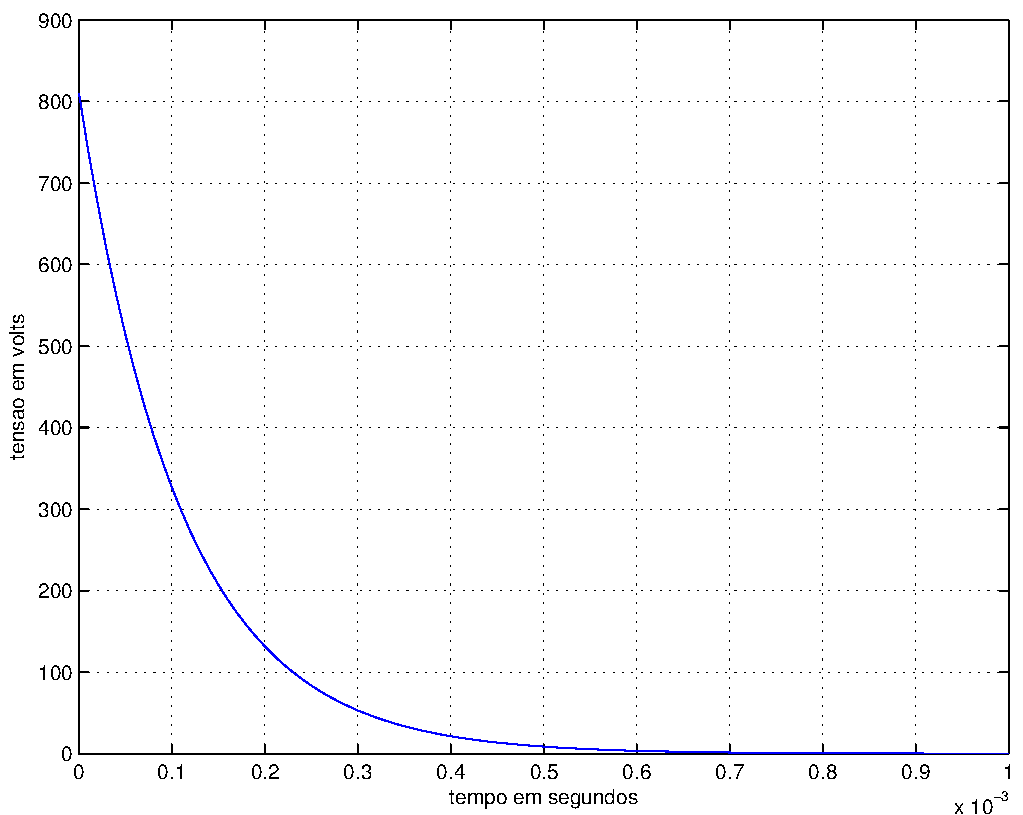
\includegraphics[scale=0.6]{expone.pdf}
    \caption{Decaimento exponencial}
\end{figure}

O ''Formigueiro'' apresenta um desafio anormal para a equipe, apresentando em todas as 
medições ruídos nos sinais de tensão e corrente. Tanto no osciloscópio ou sistema de 
aquisição. Na tentativa de encontrar o possível problema foram feitas as seguintes ações:

\textbf{Ação 0:} Retiramos o sistema de aquisição e colocamos apenas os terminais A-B na saída
da fonte. Com isto, a resposta do sistema passou a ser totalmente coerente com uma 
exponencial. 

\textbf{Ação 1:} Com a constatação vista na ação 0, mudamos todas as ligações de alimentação
dos equipamentos(fonte, osciloscópio, netbook). O sistema de aquisição foi inserido 
novamente nas medições e novamente o sinal de erro apareceu.

\textbf{Ação 2:} Explorando o conceito de ruído, o fio negativo da ponteira de tensão do
osciloscópio foi colocado em flutuação e o positivo no positivo da fonte. O pulso foi 
gerado pela fonte e NOVAMENTE o MESMO ruido apareceu. IDÊNTICO de ruido quando a ponteira
negativo esta conectado ao eletrodo \textbf{P}

\textbf{Ação 3:} Duvidamos então da continuidade do fio, que ligam as hastes B e P e 
topologia(alvo na medição de aterramento). Retornamos ao passo feito na \textit{ação 0}
e colocamos todas as possibilidades possíveis de ligação (A-B, A-P, P-B) na saída da fonte
sem o sistema de aquisição e nenhuma anomalia foi notada.

\textbf{Ação 4:} Em um determinado momento, após diversas mudança de cabos, conexões um 
sinal foi captado pelo sistema de aquisição. Sinal este que não era mais um ruído e sim
um exponencial. Entretanto com a tensão de pico baixa, na ordem de 50 V. Afastamos
os eletrodos auxiliares. A tensão de pico permanecia inalterada.

\textbf{Conclusão parcial}

\end{document}
